Vidutinis mėnesinis saulės dėmių skaičius\cite{sunspots} 1880 - 2016 metais.
Globalios mėnesinės temperatūros vidutinės anomalijos\cite{temp} tuo pačiu laikotarpiu.

\begin{figure}
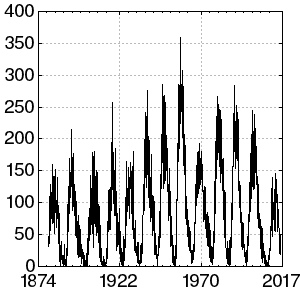
\includegraphics[scale=0.65]{../scripts/sunspots_temperature/sunspots.png}
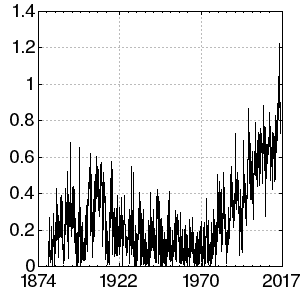
\includegraphics[scale=0.65]{../scripts/sunspots_temperature/temp.png}
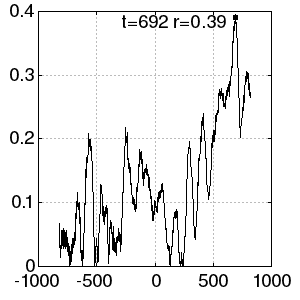
\includegraphics[scale=0.65]{../scripts/sunspots_temperature/result.png}
\caption{Grafikas kairėje: vidutinis mėnesinis saulės dėmių skaičius. Grafikas centre: globalios mėnesinės temperatūros vidutinės anomalijos. Grafikas dešinėje: signalų tarpusavio koreliacija.}
\end{figure}

Signalų poros koreliacijos funkcija rodo didžiausią signalų panašumą \( R_{fg}(t) = 0.39 \), kai \( t = 692 \).
\( R_{fg}(t)\) rodo labai silpną statistinį ryšį. O, \(t\) yra 692 mėnesiai, tai yra apie 57 metų poslinkis.
Esant tokiems rezultatams galima konstatuoti, kad koreliacijos tarp saulės aktyvumo ir temperatūros anomalijų nėra arba reikia smulkesnės analizės.
Panašias išvadas pateikia kitas tyrimas\cite{temp_study}.
Saulės aktyvumas kinta periodiškai kas vienuoliką metų. Poslinkis \(t\) turėtų būti \(< 122 \) mėnesių.
